%%% The main file. It contains definitions of basic parameters and includes all other parts.

%% Settings for single-side (simplex) printing
% Margins: left 40mm, right 25mm, top and bottom 25mm
% (but beware, LaTeX adds 1in implicitly)
\documentclass[12pt,a4paper]{report}
\setlength\textwidth{145mm}
\setlength\textheight{247mm}
\setlength\oddsidemargin{15mm}
\setlength\evensidemargin{15mm}
\setlength\topmargin{0mm}
\setlength\headsep{0mm}
\setlength\headheight{0mm}
% \openright makes the following text appear on a right-hand page
\let\openright=\clearpage

%% Settings for two-sided (duplex) printing
% \documentclass[12pt,a4paper,twoside,openright]{report}
% \setlength\textwidth{145mm}
% \setlength\textheight{247mm}
% \setlength\oddsidemargin{14.2mm}
% \setlength\evensidemargin{0mm}
% \setlength\topmargin{0mm}
% \setlength\headsep{0mm}
% \setlength\headheight{0mm}
% \let\openright=\cleardoublepage

%% Generate PDF/A-2u
\usepackage[a-2u]{pdfx}

%% Character encoding: usually latin2, cp1250 or utf8:
\usepackage[utf8]{inputenc}

%% Prefer Latin Modern fonts
\usepackage{lmodern}

%% Further useful packages (included in most LaTeX distributions)
\usepackage{amsmath}        % extensions for typesetting of math
\usepackage{amsfonts}       % math fonts
\usepackage{amsthm}         % theorems, definitions, etc.
\usepackage{bbding}         % various symbols (squares, asterisks, scissors, ...)
\usepackage{bm}             % boldface symbols (\bm)
\usepackage{graphicx}       % embedding of pictures
\usepackage{fancyvrb}       % improved verbatim environment
\usepackage{natbib}         % citation style AUTHOR (YEAR), or AUTHOR [NUMBER]
\usepackage[nottoc]{tocbibind} % makes sure that bibliography and the lists
			    % of figures/tables are included in the table
			    % of contents
\usepackage{dcolumn}        % improved alignment of table columns
\usepackage{booktabs}       % improved horizontal lines in tables
\usepackage{paralist}       % improved enumerate and itemize
\usepackage[usenames]{xcolor}  % typesetting in color

%%% Added by Janka
\usepackage{pdfpages}
\usepackage{todonotes}
\usepackage{subcaption}
\usepackage{gensymb}
\usepackage{listings}
\usepackage{forest}
\usepackage{dirtree}
\usepackage{tikz}
\usepackage{enumitem}
\usepackage{lscape}
\setlist[1]{itemsep=-2pt,topsep=3pt,parsep=3pt}
%%% Basic information on the thesis

% Thesis title in English (exactly as in the formal assignment)
\def\ThesisTitle{Visual Localization of an Object in~3D~Space}

% Author of the thesis
\def\ThesisAuthor{Jana Bátoryová}

% Year when the thesis is submitted
\def\YearSubmitted{2018}

% Name of the department or institute, where the work was officially assigned
% (according to the Organizational Structure of MFF UK in English,
% or a full name of a department outside MFF)
\def\Department{Department of Theoretical Computer Science and Mathematical Logic}

% Is it a department (katedra), or an institute (ústav)?
\def\DeptType{Department}

% Thesis supervisor: name, surname and titles
\def\Supervisor{prof. RNDr. Roman Barták, Ph.D.}

% Supervisor's department (again according to Organizational structure of MFF)
\def\SupervisorsDepartment{Department of Theoretical Computer Science and Mathematical Logic}

% Study programme and specialization
\def\StudyProgramme{Computer Science}
\def\StudyBranch{General Computer Science}

% An optional dedication: you can thank whomever you wish (your supervisor,
% consultant, a person who lent the software, etc.)
\def\Dedication{%
This thesis is dedicated to all students who were or are struggling with the
thesis as me and to their friend, families who support them. I encourage you to
not to give up and continue.

I want to acknowledge and thank my supervisor for the topic and the patience
during last two years. A great appreciation belongs to Michal Koutný as my
consultant, since he was the one who helped me with the toughest beginning. A
great appreciation belongs to my dearest Dominik Smrž since he was with me
during the dark and bright days of writing this thesis. I thank my parents, for
never-ending support. They gave me the opportunity to study. To all my friends
thank you for your understanding and encouragement in many, many moments of
crisis. Also, thank Martin Faltus for lending me a robot for the experiments.
}

% Abstract (recommended length around 80-200 words; this is not a copy of your thesis assignment!)
\def\Abstract{%
The purpose of this project is to propose and implement a system for object
localization using a stereo vision -- two cameras. The system computes the
position of the cameras relatively to each other using a calibration pattern.
Then a user selects an object to track. Different algorithms can be used for
the tracking.  The available tracking algorithms are detection-based and also
sequence-based.  When is the object found in the view of both cameras, it
estimates a position in three-dimensional space of the object using
triangulation.
}

% 3 to 5 keywords (recommended), each enclosed in curly braces
\def\Keywords{%
{3D} {localization} {tracking} {opencv}
}

%% The hyperref package for clickable links in PDF and also for storing
%% metadata to PDF (including the table of contents).
%% Most settings are pre-set by the pdfx package.
\hypersetup{unicode}
\hypersetup{breaklinks=true}

% Definitions of macros (see description inside)
%%% This file contains definitions of various useful macros and environments %%%
%%% Please add more macros here instead of cluttering other files with them. %%%

%%% Minor tweaks of style

% These macros employ a little dirty trick to convince LaTeX to typeset
% chapter headings sanely, without lots of empty space above them.
% Feel free to ignore.
\makeatletter
\def\@makechapterhead#1{
  {\parindent \z@ \raggedright \normalfont
   \Huge\bfseries \thechapter. #1
   \par\nobreak
   \vskip 20\p@
}}
\def\@makeschapterhead#1{
  {\parindent \z@ \raggedright \normalfont
   \Huge\bfseries #1
   \par\nobreak
   \vskip 20\p@
}}
\makeatother

% This macro defines a chapter, which is not numbered, but is included
% in the table of contents.
\def\chapwithtoc#1{
\chapter*{#1}
\addcontentsline{toc}{chapter}{#1}
}

% Draw black "slugs" whenever a line overflows, so that we can spot it easily.
\overfullrule=1mm

%%% Macros for definitions, theorems, claims, examples, ... (requires amsthm package)

\theoremstyle{plain}
\newtheorem{thm}{Theorem}
\newtheorem{lemma}[thm]{Lemma}
\newtheorem{claim}[thm]{Claim}

\theoremstyle{plain}
\newtheorem{defn}{Definition}

\theoremstyle{remark}
\newtheorem*{cor}{Corollary}
\newtheorem*{rem}{Remark}
\newtheorem*{example}{Example}

%%% An environment for proofs

%%% FIXME %%% \newenvironment{proof}{
%%% FIXME %%%   \par\medskip\noindent
%%% FIXME %%%   \textit{Proof}.
%%% FIXME %%% }{
%%% FIXME %%% \newline
%%% FIXME %%% \rightline{$\square$}  % or \SquareCastShadowBottomRight from bbding package
%%% FIXME %%% }

%%% An environment for typesetting of program code and input/output
%%% of programs. (Requires the fancyvrb package -- fancy verbatim.)

\DefineVerbatimEnvironment{code}{Verbatim}{fontsize=\small, frame=single}

%%% The field of all real and natural numbers
\newcommand{\R}{\mathbb{R}}
\newcommand{\N}{\mathbb{N}}

%%% Useful operators for statistics and probability
\DeclareMathOperator{\pr}{\textsf{P}}
\DeclareMathOperator{\E}{\textsf{E}\,}
\DeclareMathOperator{\var}{\textrm{var}}
\DeclareMathOperator{\sd}{\textrm{sd}}

%%% Transposition of a vector/matrix
\newcommand{\T}[1]{#1^\top}

%%% Various math goodies
\newcommand{\goto}{\rightarrow}
\newcommand{\gotop}{\stackrel{P}{\longrightarrow}}
\newcommand{\maon}[1]{o(n^{#1})}
\newcommand{\abs}[1]{\left|{#1}\right|}
\newcommand{\dint}{\int_0^\tau\!\!\int_0^\tau}
\newcommand{\isqr}[1]{\frac{1}{\sqrt{#1}}}

%%% Various table goodies
\newcommand{\pulrad}[1]{\raisebox{1.5ex}[0pt]{#1}}
\newcommand{\mc}[1]{\multicolumn{1}{c}{#1}}


% Title page and various mandatory informational pages
\begin{document}
%%% Title page of the thesis and other mandatory pages

%%% Title page of the thesis

\pagestyle{empty}
\hypersetup{pageanchor=false}
\begin{center}

\centerline{\mbox{
\includegraphics[width=166mm]{../img/logo-en.pdf}}}

\vspace{-8mm}
\vfill

{\bf\Large BACHELOR THESIS}

\vfill

{\LARGE\ThesisAuthor}

\vspace{15mm}

{\LARGE\bfseries\ThesisTitle}

\vfill

\Department

\vfill

\begin{tabular}{rl}

Supervisor of the bachelor thesis: & \Supervisor \\
\noalign{\vspace{2mm}}
Study programme: & \StudyProgramme \\
\noalign{\vspace{2mm}}
Study branch: & \StudyBranch \\
\end{tabular}

\vfill

% Zde doplňte rok
Prague \YearSubmitted

\end{center}

\newpage

%%% Here should be a bound sheet included -- a signed copy of the "bachelor
%%% thesis assignment". This assignment is NOT a part of the electronic
%%% version of the thesis. DO NOT SCAN.

%%% A page with a solemn declaration to the bachelor thesis

\openright
\hypersetup{pageanchor=true}
\pagestyle{plain}
\pagenumbering{roman}
\vglue 0pt plus 1fill

\noindent
I declare that I carried out this bachelor thesis independently, and only with the cited
sources, literature and other professional sources.

\medskip\noindent
I understand that my work relates to the rights and obligations under the Act No.~121/2000 Sb.,
the Copyright Act, as amended, in particular the fact that the Charles
University has the right to conclude a license agreement on the use of this
work as a school work pursuant to Section 60 subsection 1 of the Copyright Act.

\vspace{10mm}

\hbox{\hbox to 0.5\hsize{%
In ........ date ............	% FIXME!
\hss}\hbox to 0.5\hsize{%
signature of the author
\hss}}

\vspace{20mm}
\newpage

%%% Dedication

\openright

\noindent
\Dedication

\newpage

%%% Mandatory information page of the thesis

\openright

\vbox to 0.5\vsize{
\setlength\parindent{0mm}
\setlength\parskip{5mm}

Title:
\ThesisTitle

Author:
\ThesisAuthor

\DeptType:
\Department

Supervisor:
\Supervisor, \SupervisorsDepartment

Abstract:
\Abstract

Keywords:
\Keywords

\vss}

\newpage

\openright
\pagestyle{plain}
\pagenumbering{arabic}
\setcounter{page}{1}


%%% A page with automatically generated table of contents of the bachelor thesis

\tableofcontents

%%% Each chapter is kept in a separate file
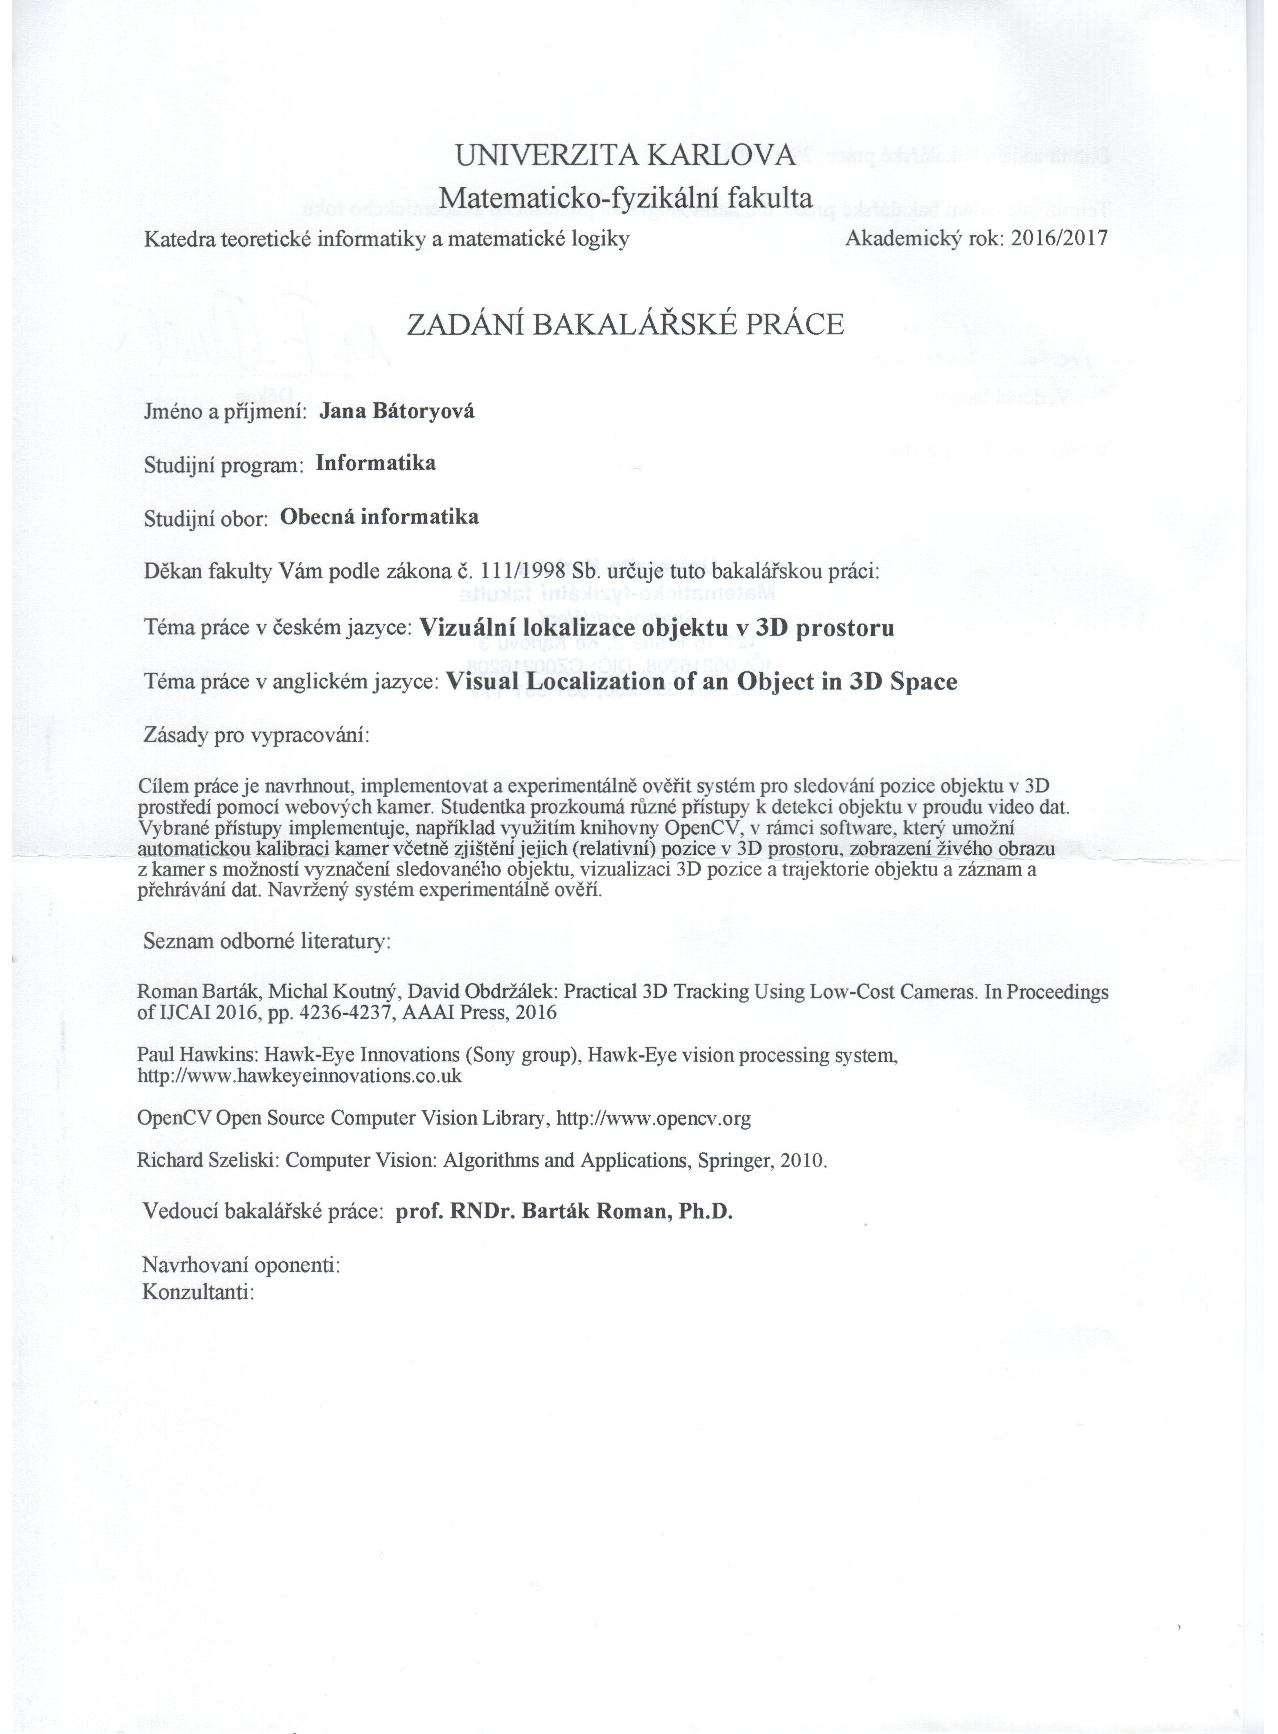
\includepdf[pages=-]{zadanie-bp}
\chapter*{Introduction}
\addcontentsline{toc}{chapter}{Introduction}

Living in the 21st century, we are witnessing a huge improvement of the
computers and their abilities. Since the beginning of the era of computers,
people have been creating machines and programs that solve problems more
efficiently than human.

From the beginning, a human has two eyes. He is equipped with stereo vision.
Moreover, man can use it from the beginning of his life. Two eyes provide
stereo vision, which is useful to estimate how far and where exactly in 3D
space is an observed object.

Our goal is to propose a system that will be capable of similar results using a
computer and web cameras. The system can be used to monitor and track movement
of the objects. For example, it can provide a trajectory of the quadcopter
flight, or another autonomous robot. These obtained data can be used for
additional analysis.

To achieve the above goal, we need to solve a problem of object detection,
tracking, and stereo vision by providing an image stream from two cameras. We
focus on an overall process from the camera calibration, through object
detection in both cameras to estimation of the object position in 3D space.

This thesis will be divided by the three steps to achieve our goal. The first
step is to obtain information about the cameras. The Calibration chapter covers the
process of obtaining a parameters to describe camera model by viewing specific
pattern. Enough images of specific pattern provide enough information to get
the parameters describing a camera.  Furthermore, positions of the pattern
where both cameras see the pattern can be used for a stereo calibration. The
stereo calibration provide information about the relative position of the
cameras to each other. This relative position and the camera parameters we will
later use in the localization process.

The second step is to track an object. Firstly, user defines the object and
then the object position estimation is provided by tracker algorithm. Many
different approaches may be used. We differenciate between the tracking
algorithms which work with a sequence of the images (sequence-based) and the
algorithms working only with one image (detection-based). We provide several
tracking algorithms from both groups. At the end of the chapter, we provide a
comparison of mentioned trackers.

The chapter Localization covers a steps needed to estimate a position of the
object in three-dimensional space. At the beginning of the chapter, we choose
and describe coordinate system, using results from stereo calibration. Then we
derive projection matrices, which transforms from the world coordinates to the
image coordinates. As a next step we introduce simple triangulation, which
estimates the position of the object in 3D by providing calibration results,
projection matrices and the coordinates of the object in both camera images.

At the end of the thesis, we provide results of an evaluation of the proposed
system. In the first experiments, we ommit a trackers and we evaluate a
accuracy of the calibration and localization. Final experiments presents
results from the tests of the program as a whole, from calibration through
tracking until localization. 

In the appendix we include user documentation for running the program and
programmer documentation for better understanding of the code.

\todo[inline]{Mozno by tu mohol zazniet aspon nastrel analyzy}
\todo[inline]{Ako stepan by som vymenovala goals}

\todo[inline]{Chyba ti cela kapitola analysis -- Problem analysis}

\todo[inline]{pridat clanok a michala bartaka a obdrzalka do referencii}
\todo[inline]{pridat opencv dokumentaciu do zdrojov}
\todo[inline]{Zadanie}

\chapter{Related works} 

The subject of retrieving an object position in 3D is well known and discussed
in many papers. Usage can be found in many different areas, for example in
sports in unclear situation, in the robotics for better navigation and
also in augumented reality for more impressive effect.

\section{Stereo vision systems}

In the paper by \citet*{zheng2010study}, the authors research stereo vision. The
proposed system has a requirement of the parallel alignment of cameras both to
each other and also parallel to the floor. The authors test the accuracy of the
system and also the disparity of the results in different distances. They
provide several experiments measuring these disparities moving an object in an
environment with one-color background.

The paper by \citet*{black2002multi} tries to solve a problem of the prediction
the object position under full occlusion. The authors of the
\citet*{yonemoto1998tracking} solve a problem of correct localization of the
object consisting of multiple parts. Such objects often fall apart when
trying to include them in virtual reality (for example a snowman can be mapped
as three balls apart of each other). The proposed system estimated parameters and
fixed points for each part independently. Then the system uses correspondence
of the points within the movements.

The system for the object tracking and localization in the garage was introduced
in the paper \citet*{ibisch2015arbitrary}. The proposed system uses a few cameras
that share parts of their views. For object detection, they use a method of the
background subtraction. Since the system's primary use is in the garage, they
also propose a method to cope with the change of lighting caused by car
lights. Their primary goal is to predict possible car collisions and therefore
to provide a data for a warning system.

\section{Use of the systems in sports}

An excellent example of an usage of a system for tracking an object in 3D space
is to solve unclear situations in sports, where sight of the naked human
eye is inconclusive. Over the last few years, one of the most famous systems is
Hawk Eye (shortly described in \citet*{owens2003hawk}). The system provides
access to the trajectory of the ball and can replay it to referees.
Furthermore, even the most popular soccer competitions are experimenting with
the system for detecting if the ball crosses the goal line or not.  This system needs
an expensive setup equipped with high-speed cameras an the software itself is of
high price.

\section{Use of the systems in robotics}

The principles described in previous sections have a extensive usage in
robotics, for better navigation, object manipulating and so on. For example,
for the robotic competition
RoboCup, the category Soccer many systems for ball tracking were developed. Robots
competing in this category are usually equipped with an omnidirectional camera.
This camera is pointing vertically up, where the image reflects in a mirror.
This principle provides a full 360\degree image of the environment provided by
only one camera. In this case, it is possible to track an object by single
camera, since additional information about the ball (such as color and size)
is provided in advance. On the other hand, such a system is not static, the
background changes with every movement of the robot. Nevertheless, usage of
additional camera may significatly improve the precision. For more information
about it, we refer to the paper \citet*{kappeler20103d}.


\section{Dove-eye}

The idea of this work is based on its predecestor, Dove-eye presented in the
paper by \citet*{dove-eye}. This project use automatic calibration process, to
get the infromation about the cameras and provide a several ways to track an
object. Localization results are displayed live.

\section{Our approach}

Starting with the ideas used in Dove-eye, we developed a new implementation for
this task. We improve the the tracking process by providing many different
trackers, which give an opportunity to choose the one which is best suitable for
given environment. We provide an easy way to correct the tracker by its
reinitialization. Furthermore, no knowledge of the internals is needed to add a
new tracker.  In difference to some previously mentioned papers, we do not
require special alignemt of the cameras. 

We also implement an similar algorithm to the one mentioned by
\citet*{ibisch2015arbitrary} and others. As opposite to paper by
\citet*{kappeler20103d} we do not use any previous information about the object
tracked.

This thesis also considers a case of tracking multiple objects. It provides a
way, to initialize tracking objects. The comparison of the trackers is
provided, including their speed, accuracy, but also ability to track
multiple objects.

We conclude the thesis with several experiments, including ones with autonomous
robot, to test the system suitability for an use in the robotics.

\chapter{Proposed system}

To be able to locate an object in 3D with no previous knowledge of the object (such
as its size, color and so on), two views of the same object are needed. The
views can be obtained by one moving camera or by multiple cameras. In this
thesis, we take a closer look at the second approach.

We propose a system with two cameras, connected via USB to a computer.
Two cameras provide enough information for object localization and make the
project usable also on low-budget. The placement of the cameras is important,
but no precise alignment is required. The cameras should share a significant part
of the view (see an example of the setup in the Figure \ref{fig:camera-setup}).

\begin{figure}
	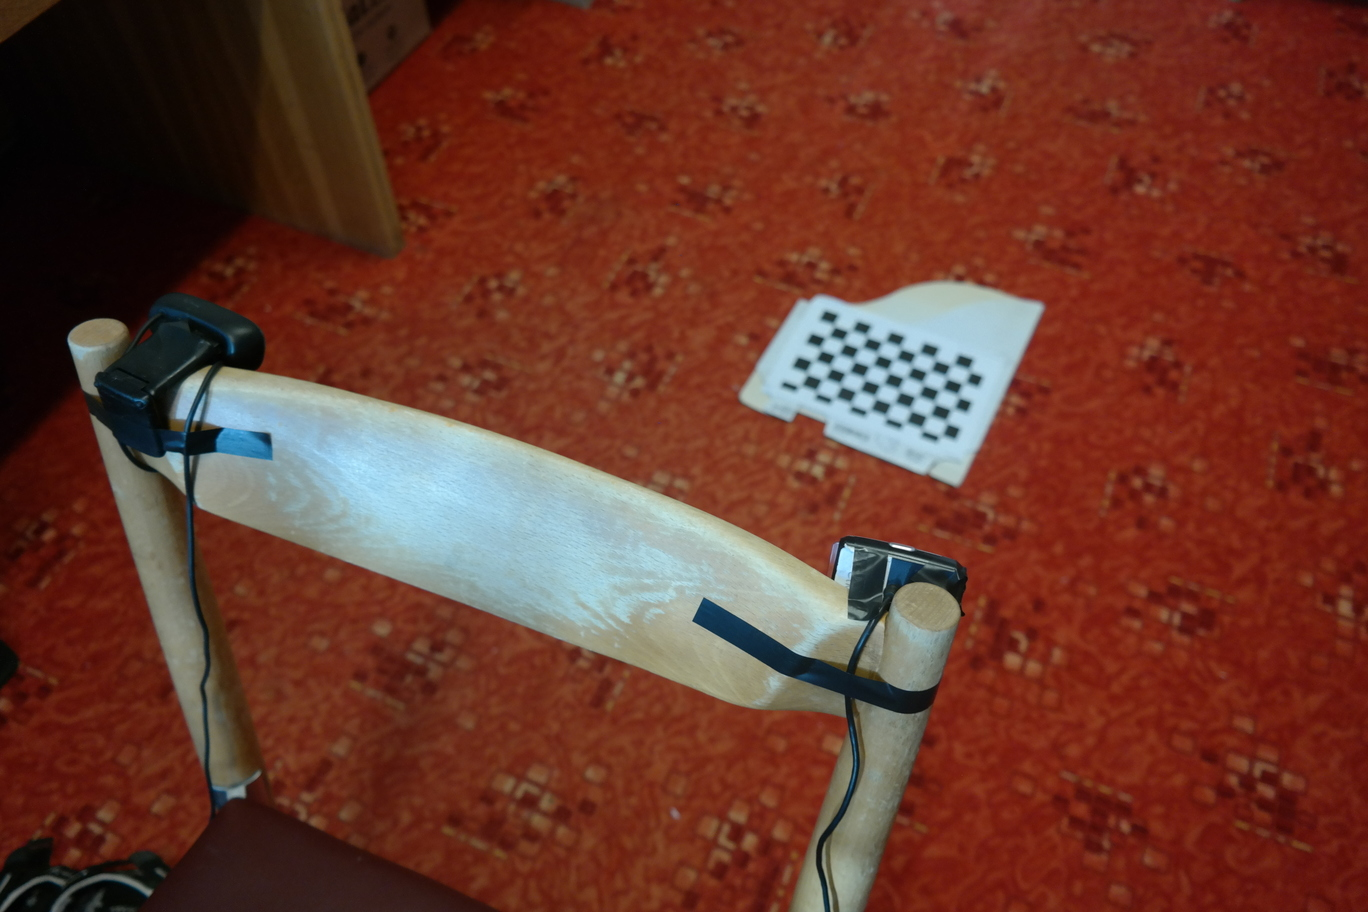
\includegraphics[width=\linewidth]{img/camera-positions.jpg}
	\caption{Example of camera setup}
	\label{fig:camera-setup}
\end{figure}

The program will be able to calibrate cameras to get their parameters. This
calibration will be based on showing a specific pattern to both cameras. From
this calibration, we obtain information for both cameras, but also their
distance to each other and the rotation between them.

After this calibration, the user marks the objects in both views of the
cameras. At this point, the tracker will start to estimate an object position
in camera view based on the images. We provide different tracker, so the user
can choose one to work with.

When we obtain information from calibration and the object position from both
images, we will estimate the object position in 3D space by simple linear
triangulation.

The each described step is crucial to get a system, which will be able to
localize point in 3D space. Each step is discussed separately in the following
chapter.

Now we provide a short insight into used tools and the notations, which are
used to describe our solution to the problem.

\section{Tools}

For the computer vision task, we use an \emph{OpenCV} library. OpenCV is an open
source computer vision library with many algorithms implemented (for example
calibration, triangulation, and so on). We use trackers which are now available
only in the \emph{contribute} version. For more information and examples of usage
visit their webpage\footnote{\url{https://opencv.org/}}.

To provide a comparison of trackers, we also include one tracker from
\emph{Dlib}\footnote{\url{http://dlib.net/}} library. It is also open source
and an interface for the Python is provided.  Since this library focus is on
machine learning, it does not contain as many functions for computer vision
as the OpenCV library yet.

\section{Notations}

The following section describes some procedures using math notion. To avoid
ambiguity we provide the overview of the used notation here.

\subsubsection*{Vector}
A word \emph{vector} denotes a column vector in a shape of $n\times1$.

\subsubsection*{Block matrix}
A matrix operation $W = (A|B)$, where $A$ is a matrix $m \times n$ and B is a
matrix $m \times p$, creates matrix $W$, where the first $n$ columns are the entries from
matrix $A$ and the last $p$ columns consist of the columns of matrix $B$.
Example:

\[
A = \begin{pmatrix}
        1 & 2 \\
        3 & 4
\end{pmatrix},
B = \begin{pmatrix}
5 \\
6
\end{pmatrix},
(A|B) = \begin{pmatrix}
        1 & 2 & 5 \\
        3 & 4 & 6
\end{pmatrix}
\]

\subsubsection*{Homogeneous coordinates}

In computer vision, homogeneous coordinates are used frequently instead of
Cartesian coordinates. Cartesian coordinates are the most common coordinate
system.  Homogeneous coordinates have one element added. This element is a
scaling factor. As an example, vector $(2x, 2y, 2z, 2)^T$ represents same point
as $(x, y, z, 1)^T$ in homogeneous coordinates. The same point is equal to $(x,
y, z)^T$ in Cartesian coordinates. Unlike the Cartesian coordinates, a single
point can be represented by infinitely many homogeneous coordinates.

Similarly it works for coordinates in any n-dimensional space. In conversion
from Cartesian to homogeneous coordinates we simply add a new element at the end
equal to one. In the opposite direction, we divide first $n-1$ values by the
$n$th.

In homogeneous coordinates the origin is left out. Homogeneous coordinates provide
us also a way how to represent a point in the infinity by finite coordinates.
These points in the infinity are represented with the scale factor equal to 0.

This coordinates representation is tightly bounded to a projective plane, on
which the mathematical theory behind is based. For us, it is just important to
know how to convert them to Cartesian coordinates and that algorithms for
computer vision often use them.

\chapter{Calibration}

Our goal is to create a system which does not need any prior information about the
position of cameras. Since we do not know how far away the cameras are, nor
angles between them, we firstly use calibration to obtain this information.

By calibrating cameras with a well describable pattern, we can obtain
information about the single camera, such as what distortion its lens cause, or
how the world points are projected to an image plane of the camera.

After discovering these parameters for both cameras, we will continue on stereo
calibration. Stereo calibration will provide us information about their
position in space relative to each other.

For these calibration processes, we use algorithms implemented in OpenCV.
Therefore, we provide only a short overview of the process, and we describe
only results obtained from calibration essential to us.

\section{Intrinsic parameters}

Each camera type is different. Moreover, each camera of a specific type is
different due to a manufacturing process. Therefore we introduce intrinsic
camera parameters, which help us to model the camera precisely.

Intrinsic camera parameters define a transformation between the world coordinates and
the coordinates within an image plane (in pixels). Physical attributes of the
camera influence this transformation.

These parameters include focal length, a position of the principal point and
distortion coefficients. All these parameters are needed to get a correct
transformation between the point in the space and the point at the image plane.
Sometimes even more parameters are used for a better description of the model
of the camera.

\subsection{Camera matrix} 

Camera matrix will provide us a transformation from
world coordinates (with the origin in the camera) to image plane coordinates
(seen in the image taken from the camera). If the coordinates in 3D are
available, we can obtain 2D coordinates by simple multiplication by camera
matrix. After multiplication we obtain 2D homogeneous coordinates.

As the next step, we describe the camera matrix obtained by OpenCV calibration
procedure. In the OpenCV implementation the camera matrix is $3\times3$ matrix of the
following format:

\[
\begin{pmatrix}
	f_x 	& 0 	& c_x \\
	0	& f_y	& c_y \\
	0	& 0	& 1
\end{pmatrix}
\]

Where $f_x$, $f_y$ denote focal lengths expressed in pixel units. It is usual
to introduce two of them, separately for both axes, since pixels usually are
not perfect squares but rather rectangles. Therefore the same focal length, has
different length in pixel units over a given axis.

We refer the ray of the view of the camera as the principal ray. The point
where this ray intersects the image plane is called principal
point\footnote{For more information visit \url{https://en.wikipedia.org/wiki/Pinhole\_camera\_model\#The\_geometry\_and\_mathematics\_of\_the\_pinhole\_camera}}.
Parameters $c_x$ and $c_y$ define coordinates of the principal point in the
image plane.  It should be the center of the image, but assembling process of
the camera might cause a small displacement.

\subsection{Distortion coefficients}

Cameras are equipped with lenses to obtain sharp image instead of blurry. The
lens may causes various distortions. Fish-Eye lenses are known for their
distortion.  Even web camera lenses have distortion, but not as visible as the
camera with a fish-eye lens. It is important to correct these distortions.

Two distortion types cause a significant effect on the image. The first one is
the radial distortion, creating barrel effect and the second one tangential distortion.

The radial distortion is caused by the camera lens (the effect of radial
distortion is displayed in the image \ref{fig:distortion}). It can usually be
described by three parameters. Highly distorted images (like from fish-eye)
often need more parameters. Since our system use web cameras, we will use only
three parameters.

In the ideal camera, the lens would be placed parallel to the chip. Since such
precision is not possible, due to an assembling process, tangential distortion
arises. For this distortion, we use two parameters.

We describe both distortion effects by five parameters. More about the meaning
of the parameters could be found in the book by \citet*{bradski2008learning}.

\begin{figure}
	\begin{subfigure}[b]{0.48\linewidth}
		\includegraphics[width=\linewidth]{img/chessboard/7x8chessboard-positivedistortion}
		\caption{Effect of positive radial distortion}
	\end{subfigure}
	\begin{subfigure}[b]{0.48\linewidth}
		
\includegraphics[width=\linewidth]{img/chessboard/7x8chessboard-negativedistortion}
		\caption{Effect of negative radial distortion}
	\end{subfigure}
	\caption{Effects of lens distortion on the image of the chessboard}
	\label{fig:distortion}
\end{figure}

These nine parameters (four for camera matrix and five for distortion
coefficients) describe the camera model. They may be used for example for
projecting a point from 3D space to image coordinates in the camera (OpenCV
function \verb+projectPoints+). We will use them to get better results for
stereo calibration and for localization, since they provide us a more accurate
model of the camera.

%We can now describe the transformation process in one camera by multiplication by
%the camera matrix and then correcting the results by distortion coefficients. With
%these parameters, we can continue on stereo calibration.

%\todo[inline]{Ale co se pronasobi tou matici?}
%\todo[inline]{Napis sem ten vzorecek}

\section{Stereo calibration}

After performing a calibration of both cameras separately, we also need
information about their relative position to each other. By the relative
position, we understand translation from the first camera to the second and the
rotation of the camera (among three axes). Using this information, we can
transform a view of the one camera, by moving it by translation vector and
rotating accordingly. Therefore, the position of the second camera can be
described by six parameters, three as an angle around each ax to rotate and
three for translation vector in respect to the first camera.

Stereo calibration routine in OpenCV can also perform mono calibration for both
cameras, but we pre-calibrate cameras on itself for better precision and better
convergence of the algorithm.

Stereo calibration routine will provide more information. For the goals of this
thesis, only rotation matrix and translation vector are important.

\section{Calibration process}

In previous sections we shortly discussed theoretical background behind the
calibration. In this section we will focus on the implementation.

In OpenCV a chessboard is commonly used, since it is a planar object (easy to
reproduce by printing) and well described. OpenCV also provides methods for
automatic finding of the chessboard in the picture, so no human intervention is
needed to select the chessboard corners from the image (an example of the
chessboard is provided in a Figure \ref{fig:chessboard}). Therefore, we also
use the chessboard pattern for calibration.

\begin{figure}
	\centering
	
\includegraphics[width=0.8\linewidth]{img/chessboard/7x8chessboard}
	\caption{Example of $7\times8$ chessboard used for the calibration}
	\label{fig:chessboard}
\end{figure}

\subsection{How many images?} 
\todo[inline]{Nejak nazov bez otaznika?}

Now we know that, we can use a chessboard to calibrate the cameras. However,
the question of how many images are needed for the calibration remains. We
discuss only the images where the full chessboard is found. For enough
information from each image, we need a chessboard with at least $3\times3$
inner corners. It is better to have a chessboard with even, and odd dimension
(for example 7$\times$ 8 inner corners) since it has only one symmetry axis,
and the pose of the object can be detected correctly. It is important that the
chessboard indeed has squares, not rectangles (so it is better to check it
after printing). A bigger chessboard is easier to recognize, so we recommend at
least format A4.

We need only one image for computing the distortion coefficients. However, for
the camera matrix, we need at least two images. For stereo calibration, we need at
least one pair of images of the chessboard.

We know the minimum number of images needed for calibration. On the other hand,
we use more images for the robustness of the algorithm. We need a "rich" set of
views. Therefore it is important to move the chessboard between snapshots. With
more provided information to the algorithm, it compensates the errors in the
measurements (like a wrongly detected chessboard in one of the images).
Therefore also the computation time increases. Since it is enough for a given
setup of the cameras to perform a calibration only once and then use results
from it again, we recommend to do the calibration on more images and wait a
little bit longer for the results. 

\chapter{Tracker}

We considerate tracker as an algorithm used to detect a position of the object in
an image. We will present few tested trackers and their results in this task.
Firstly we provide a short description of simple straightforward tracker and
then we will describe more complicated trackers.

We use a word tracker generally for an algorithm able to detect object. Some
trackers but do not take an advantage of past images and information gained
from them. They simply detect an object in the each image. On the other hand
many good trackers using also information from previous images exist. For this
task some trackers from both categories.

%%%%%%%%%%%%%%%%%%%%%%%%%%%%%%%%%%%%%%%%%%%%%

\section{Simple Background Tracker}

This tracker takes a photo of the background at the beginning and calls it
\emph{pattern}. In order to detect an object in \emph{image} is taken a
comparison of the \emph{image} and \emph{pattern}. A Comparison is done by
taking a sum of an absolute difference for each colour (Red, Green, Blue) in
the images. 

As result, we get a map, where higher values mean bigger difference between the
colors of the \emph{pattern} and \emph{image} at given point. We will assume it
is caused by an object in front of the camera at given point.  As the next step
we will binarize the map with a given \emph{treshold}. At this point we will
find a countour with biggest area using OpenCV library. Centerpoint of the
rectangle of this contour will be estimated position of our object in the
image..

\todo[inline]{Pomôže práve popísaný postup zapísať v niekoľkých riadkoch pseudokódu? Bolo
by to prehľadnejšie (na jedno pozretie jasné, bez čítania odstavca, ak čitateľ
vie, čo očakávať)}

\todo[inline]{Fotka vzoru (farebne), fotka s objektom, absolute\_diff, výsledok po rôznych tresholdoch}

\todo[inline]{Nájdenie contúr na obrázku, zobrazenie najväčšej, bod ako stred}

\subsubsection{Advantages}
\begin{itemize}
\item Quite straight-forward implementation
\item Ability to recognise variate object without having specific color or pattern.
\end{itemize}

\subsubsection{Disadvantages}
\begin{itemize}
\item Cannot recover from even small movement of the camera.
\item Moving object with a hand will cause recognizing the hand also as an object and will result wrongly estimated center of the moving object. Same problems cause shadows.
\end{itemize}

%%%%%%%%%%%%%%%%%%%%%%%%%%%%%%%%%%%%%%%%%%%%%

\section{Adaptive Background Tracker}

In order to make our background tracker robust to small movement of camera we
are going to update our \emph{pattern}. This could be simply done by defining \emph{pattern}
as the mean of last \emph{n} images.

\subsubsection{Advantages}
\begin{itemize}
\item Robust against movements of the camera
\end{itemize}

\subsubsection{Disadvantages}
\begin{itemize}
\item If the object is not moving it will disappear as becoming a part of the background. After moving it will recover correctly.
\end{itemize}

%%%%%%%%%%%%%%%%%%%%%%%%%%%%%%%%%%%%%%%%%%%%%

\section{More advanced trackers}

%%%%%%%%%%%%%%%%%%%%%%%%%%%%%%%%%%%%%%%%%%%%%

\section{Comparison of trackers}

\subsubsection{Experiment with simplyfied environment}

Given a video sequence XYZ second long we studied an accuracy of trackers. The background is one colored and moving object is a red circle.

\todo[inline]{ Robot sledujúci čiaru do štvorca s červeným kruhom z vrchu (kamery sa dívajú zvrchu). Porovnanie bude uvedené ako čiary, ktoré sú nakreslené pomocou zachytených bodov.}

\subsubsection{Experiment in complex environment}

Background consistsed of many colors and patterns. Moving object has a pattern and is partially colored as the background.

\todo[inline]{ Vyskytli sa veci, ako, že stratil polohu? V akom percente? Mám ako rozumne vyjadriť presnosť tých súradníc lepšie než od oka?}

\chapter{Localization}

In the previous chapters, we have covered the steps to obtain a position of
an object in 2D images. In this chapter, we will take a closer look at
obtaining a position of an object in the world coordinates by combining
information from multiple cameras.

At this point we have computed not only intristic matrices of the cameras but
also the rotation matrix and the translation vector (from the mono camera
calibration and stereo calibration). Our goal is to get a position of the
object in world coordinates from a tuple of coordinates from the images taken by
cameras.

\section{Projection matrices}
Projection matrices provide us a way to transform world coordinates to image
coordinates. The first step is to find out projection matrices for both
cameras, and then we will use them for solving the triangulation problem.

We define a projection matrix as a transformation matrix $P$, such that: $x = P
\dot X$, where $X$ denotes a vector of size 4$\times$1 -- homogenous world coordinates
of the object and $x$ denotes homogenous object coordinates in the image plane
of the camera -- a vector 3$\times$1.

\subsection{World coordinate system}
We define the world coordinate system as orthogonal, with the origin in the
center of projection of the first (usually left) camera. The positive part of
the z-axis is pointing in front of the camera and below the camera is positive
y-axis and to the right is positive x-axis. Layout and the coordinate system is
displayed in the figure \ref{fig:coordinate-system}.

\begin{figure}
\centering
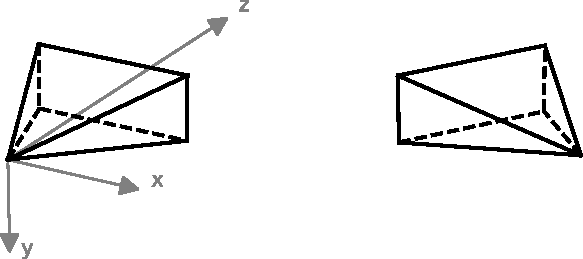
\includegraphics{img/camera-positions}
\caption{Cameras layout and coordinate system}
\label{fig:coordinate-system}
\end{figure}

\subsection{Computing projection matrices}
After defining coordinate systems, we can compute the projection matrices for
both cameras. We use projection matrix decomposition to get the projection matrix
from calibration results.

We decompose projection matrix as $P = K[R|T]$, where $K$ is intristic
camera matrix and $[R|T]$ is extrinsic matrix. $R$ is a rotation matrix and
$T$ is a translation vector. We use this decomposition to compute the projection
matrices.

\emph{First camera}
Since we set the origin of the world coordinate system in the first camera,
the camera has no rotation nor translation to the coordinate system. Therefore
we compute a projection matrix as:

\[
 P_1 = K_1 \cdot \begin{pmatrix}
	I_3 & | & 0_3  
\end{pmatrix}
\]

Where $K_1$ denotes first camera intrinsic parameters matrix, $I_3$ identity
matrix 3$\times$3 and $0_3$ zero vector. Only intristic parameters matrix take
effect on given coordinates, computing from world coordinates in the image plane of the camera.

\emph{Second camera}
For the second camera projection matrix, stereo calibration results will be
used. We know the rotation matrix and translation vector between the cameras,
being able to get coordinates of the second camera relative to the first one.

We now use this information in construction of projection matrix. $P_2 = K_2
\dot [R | T]$, where $K_2$ is second camera intristic parameters matrix, $R$
rotation matrix and $T$ translation vector.

More about the decomposition itself could be found in an article by
\citet{computervisionblog}.

\todo[inline]{V programme aktualne nerobim s distortion coeffs, pretoze uz aj bez toho su rozumne vysledky}

\section{Triangulation}
Now when we know the projection matrices we can formalize our problem as
\begin{equation}
x_1 = P_1X, x_2 = P_2X \label{projection-statements}
\end{equation}
with the goal to find $X$. Since errors may occure during
measurement of $x_1$, $x_2$ and calibration. In further steps we consider that
calibration results are provided with high accurancy compared to measurement of
$x_1$ and $x_2$ (that is the reason to have longer calibration with more images
at once).

\subsection{Simple linear triangulation}
We will now shortly describe how the triangulation is working under the hood.

The results of cross product of vector itself is zero vector. We can write
equation \ref{projection-statements} as crossproduct $x \times (PX) = 0$. We
denote point $x = (x, y, w)$, where $w = 1$ since these coordinates are
homogenous -- in other words up to scale factor $w$.

\todo[inline]{FIX x=(x...)}

We can then rewrite $x \times (PX) = 0$ in the following way:

$$ w(p^{3T}X) - x(p^{2T}X) = 0 $$
$$ y(p^{3T}X) - w(p^{1T}X) = 0 $$
$$ x(p^{2T}X) - y(p^{1T}X) = 0 $$

Where $p^{iT}$ denotes ith row of $P$. Since $w = 1$ we can equally write:

$$ x(p^{3T}X) - (p^{1T}X) = 0 $$
$$ y(p^{3T}X) - (p^{2T}X) = 0 $$
$$ x(p^{2T}X) - y(p^{1T}X) = 0 $$

These equations are linear in the components of X. Only two equations are
linearly independent since the third one could be obtained as the sum $y$
times the first row and $-x$ times the second row.

Therefore an equation of form $AX = 0$ can then be composed using two points $x_1 = (x, y, 1)$ and $x_2 = (m, n, 1)$:

\[
A = \begin{pmatrix}
x(p_1^{3T}X) - (p_1^{1T}X) \\
y(p_1^{3T}X) - (p_1^{2T}X) \\
m(p_2^{3T}X) - (p_2^{1T}X) \\
n(p_2^{3T}X) - (p_2^{2T}X) \\
\end{pmatrix}
\]

For each image two equations were included, giving a total of four equations in
four homogeneous unknowns.

Without an error during measurements a point $X$ satisfying $AX = 0$ would
exist. However, due to the errors it might not exists. As the next step, Homogenous
method (DLT) is used to find the solution. More about the method could be found
in \citet*{multiple-view-geometry}.

\section{Implementation note}
For the triangulation we used OpenCV function triangulatePoints($P_1$, $P_2$,
$x_1$, $x_2$), which is based on simple triangulation method with use of DLT
method for solving equations.

\chapter{Experiments} 

For the designed system we haven chosen multiple experiments to
verify its accuracy. Experiments in this part focus on the localization process
and overall experiments. The tracker experiments are located in the chapter
\ref{ch:tracker}.

\section{Calibration and localization}
\label{s:experiment-static}

In order to measure a quality of calibration and localization we exclude a
tracking component. Therefore, we propose an experiment with static points in a
camera views. Then we estimate a position in 3D for these points.

It is complicated to measure distance from the origin of the coordinate system,
i.e. point inside the first camera to any given point. Therefore, we measure
distances between the static points in the real world and compute the distance
between their estimated position in 3D coordinates. Then we compare the results.

To skip the tracking part, we created a new tracker.  The new tracker always
returns the same position.  Doing this, we excluded tracker from our process.

We have chosen the grid as in the figure \ref{fig:grid} as our pattern for experiments.
The vertical lines are circa 400~mm long and the distance between them is circa
200~mm. We measured distances between the crossings. We numbered the crossing,
the left column is from top to the bottom from 1 to 7 and the right column from
8 to 14 (see the figure \ref{fig:ladder_numbered}).

The setup of the cameras was nearly parallel, which means, the center rays of
their views were parallel, looking in same direction.The distance between them
was circa 16~cm. Selected points are displayed in the figure
\ref{fig:ladder_ground}. The results from this experiment are listed in the
table \ref{table:distances}. 

From the results we can see that results for horizontal lines (with the length
400~mm, third part of the table) are very accurate. On the other hand, the
results for the vertical lines were quite unstable. Based on the measured
distances between the points in the left column (first part of the table) it
seems, that results get worse when, the points are further away from the
camera. But the results computed for the points from right column bring the
hypothesis into question. 

\begin{table}
\centering
\begin{tabular}{|r|r|r|r|r|}
\hline
From	& To	& Real length (mm) & Computed length(mm) & Error (\%) \\
\hline
\hline
\input{distances.txt}
\hline
\end{tabular}
\caption{Results of the experiment focused on the distances}
\label{table:distances}
\end{table}

We were interested if the results are good not only on the one plane -- in our
case the ground -- but also in the others. Now we have tested the precision in
two axes, which were perpendicular to each other (vertical and horizontal
lines). We have noticed, that the results for the vertical lines are less
precise. Therefore, we decided to test the last axis and its precision. We places
a wall with the marks, which is perpendicular to the ground and measured the
distance between the marks. The setup can be seen in the figure
\ref{fig:table}. The marks are numbered as displayed in the image
\ref{fig:tablenumbered}. The results are included in the table
\ref{table:distances}. 

We did the same experiment with another setup, when the cameras were 63~cm
apart from each other. We were interested, if the results are better in
parallel setup, or not. Based on the results there is no evidence of the
different precision and the differences may be still caused by different
precision of the calibration. The results for this second experiment are listed
in the appendix in the table \ref{table:distances-second}. Same numbering of
the marks was used.

\begin{figure}
\centering
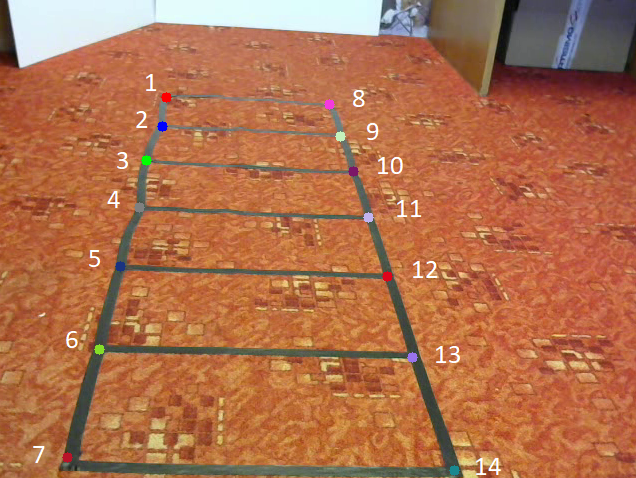
\includegraphics[width=0.8\linewidth]{img/experiments/right-ladder-numbered.png}
\caption{Numbering the points}
\label{fig:ladder_numbered}
\end{figure}

\begin{figure}
\centering
\begin{subfigure}{0.48\linewidth}
	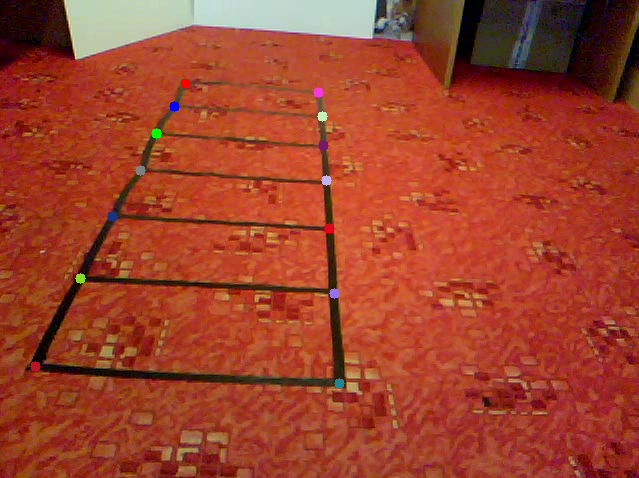
\includegraphics[width=\linewidth]{img/experiments/left-ladder.png}
\end{subfigure}
\begin{subfigure}{0.48\linewidth}
	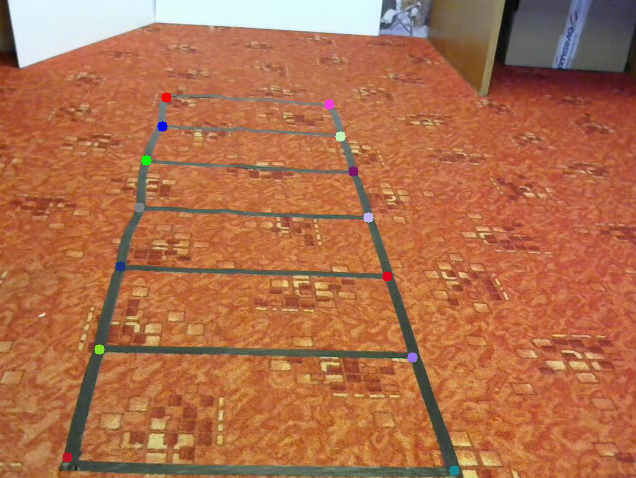
\includegraphics[width=\linewidth]{img/experiments/right-ladder.png}
\end{subfigure}
\caption{Selecting the points from the videos}
\label{fig:ladder_ground}
\end{figure}



\begin{figure}
\centering
\begin{subfigure}{0.48\linewidth}
	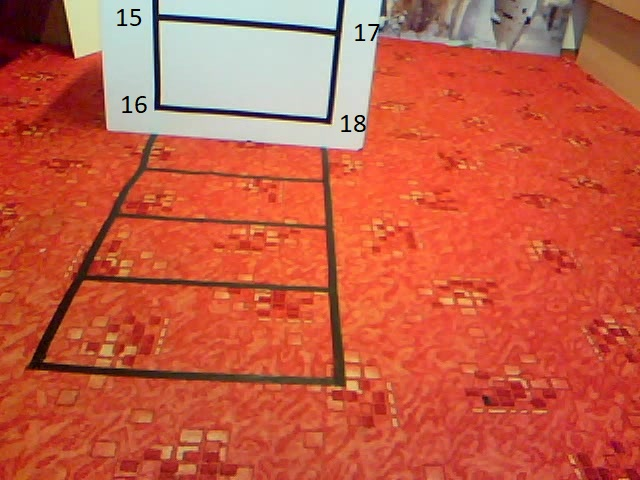
\includegraphics[width=\linewidth]{img/experiments/table-left.jpg}
	\caption{Left view of the camera with marks}
	\label{fig:tablenumbered}
\end{subfigure}
\begin{subfigure}{0.48\linewidth}
	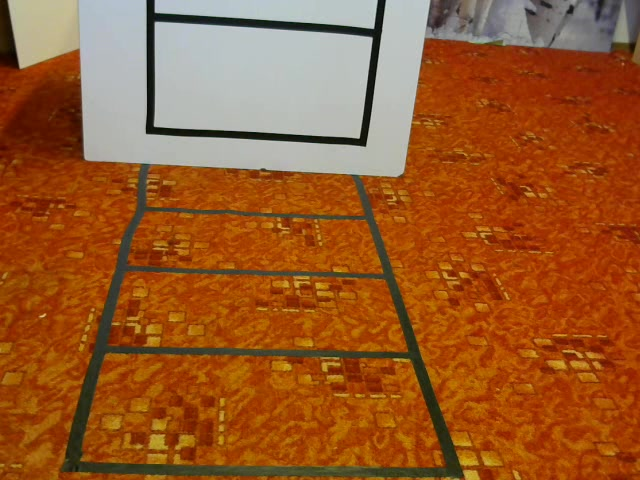
\includegraphics[width=\linewidth]{img/experiments/table-right.jpg}
	\caption{Right view of the camera}
\end{subfigure}
\caption{The views of the camera on the perpendicular plane to the ground}
\label{fig:table}
\end{figure}

\begin{figure}
\centering
\begin{tikzpicture}[]
	\draw (0, 0) -- (12, 0);
	\draw (0, 4) -- (12, 4);	
	\draw (0, 0) -- (0, 4);
	\draw (2, 0) -- (2, 4);
	\draw (4, 0) -- (4, 4);
	\draw (6, 0) -- (6, 4);
	\draw (8, 0) -- (8, 4);
	\draw (10, 0) -- (10, 4);
	\draw (12, 0) -- (12, 4);
	\node [right] at (0.1, -0.25) {200mm};
	\node [right] at (2.1, -0.25) {200mm};
	\node [right] at (4.1, -0.25) {200mm};
	\node [right] at (6.1, -0.25) {200mm};
	\node [right] at (8.1, -0.25) {200mm};
	\node [right] at (10.1, -0.25) {200mm};
	\node [right] at (12.1, 2) {400mm};
\end{tikzpicture}
\caption{Pattern used for experiments}
\label{fig:grid}
\end{figure}

\section{Complex experiments}

As the last step, we decided to test whole system in a real environment. This
time we included all parts of the application -- calibration, tracking and also
localization. In the previous experiments, we tested the liability of the
trackers and the precision of the results. Now we test the usability of the
system as the whole.

\subsection{Experiment with the one small object}

The most important experiment -- the experiment which decides if the system is
usable -- is experiment under real conditions. We created for our autonomous
robot a square to follow, with the length of the side equal 14.5~cm (see figure
\ref{fig:robot-square}). The robot did four laps around the square. The
results are displayed in the figure \ref{fig:square-results}.

We can see in the left picture, that the drawn line is similar to our shape.
Not having sharp edges, since our robot make a small arc. On the other hand,
the results from the another view are not so amazing. The coordinates have a
lot of noise over Z-axis. The noise is only present, if the robot is following
horizontal lines of the square. As the last step we computed maximum of the
distances between any two points, which were located. In this case, the ideal
value would be the length of the diagonal, which is equal to 20.5061~cm. Our
results are between 18.54~cm to 19.38~cm, depending on the run. That means,
that the error is only usually between 1 and 2~cm.

\begin{figure}
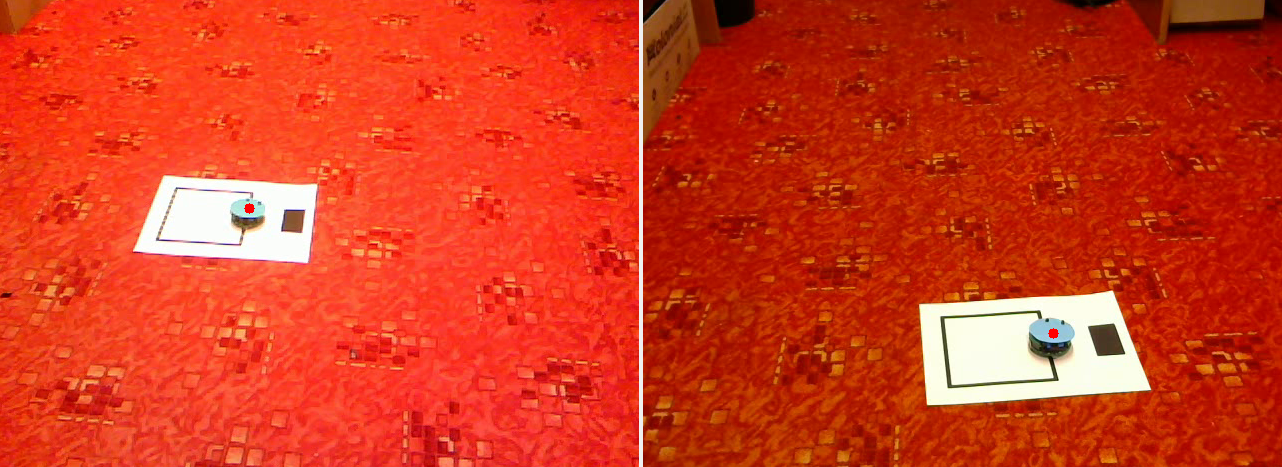
\includegraphics[width=\linewidth]{img/experiments/square-robot.png}
\caption{Experiment with the robot}
\label{fig:robot-square}
\end{figure}

\begin{figure}
\centering
\begin{subfigure}{0.48\linewidth}
	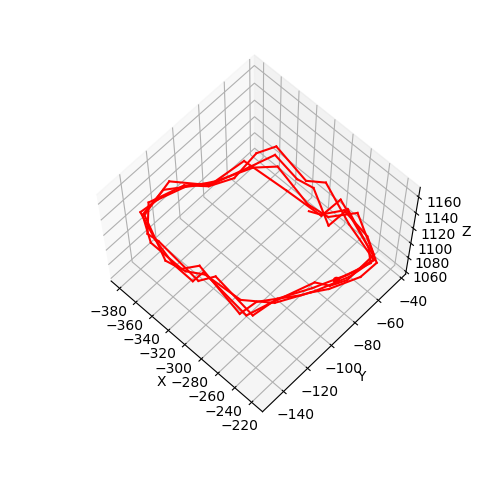
\includegraphics[width=\linewidth]{img/experiments/square-nice.png}
\end{subfigure}
\begin{subfigure}{0.48\linewidth}
	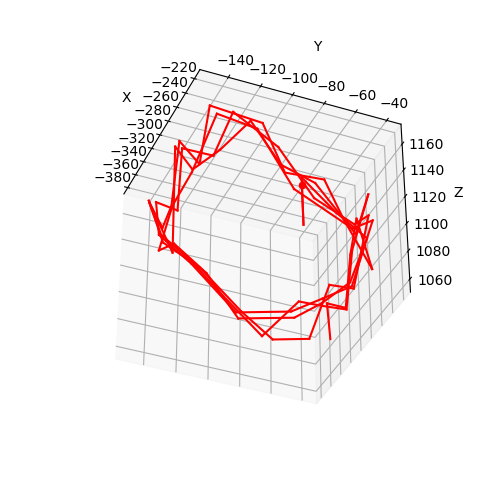
\includegraphics[width=\linewidth]{img/experiments/square-ugly.png}
\end{subfigure}
\caption{Results of the localization -- four laps by the robot}
\label{fig:square-results}
\end{figure}

\subsection{Experiment with two objects}

This experiment will test the ability of the system to track multiple objects.
This effectively exclude \simback{} tracker as it is not able to track multiple
objects. Furthermore, we track objects with multicolored surface, making \hsv
tracker also unusable. The rest of the trackers are mostly slower, more
problematic.

We can see the setup for the experiment in the figure \ref{fig:two-init}. We
can see two boxes, both in shades of blue. During testing many trackers failed
to track the object and lost it. We chose the \corr{} tracker as it provided
best results. It is medium fast tracker. The tracker sometimes lost the
images, but most of the time it was able to track. Because of the object lost,
sometimes an interaction of the user is needed, to reinitialize a tracker.

Sample results of the trajectories for two objects is displayed in the figure
\ref{fig:two-trajectories}. During the experiment, the boxes were moving
between the yellow marks and swapped places. We can see these four marks also in
both trajectories quite close to each other. 

\begin{figure}[p]
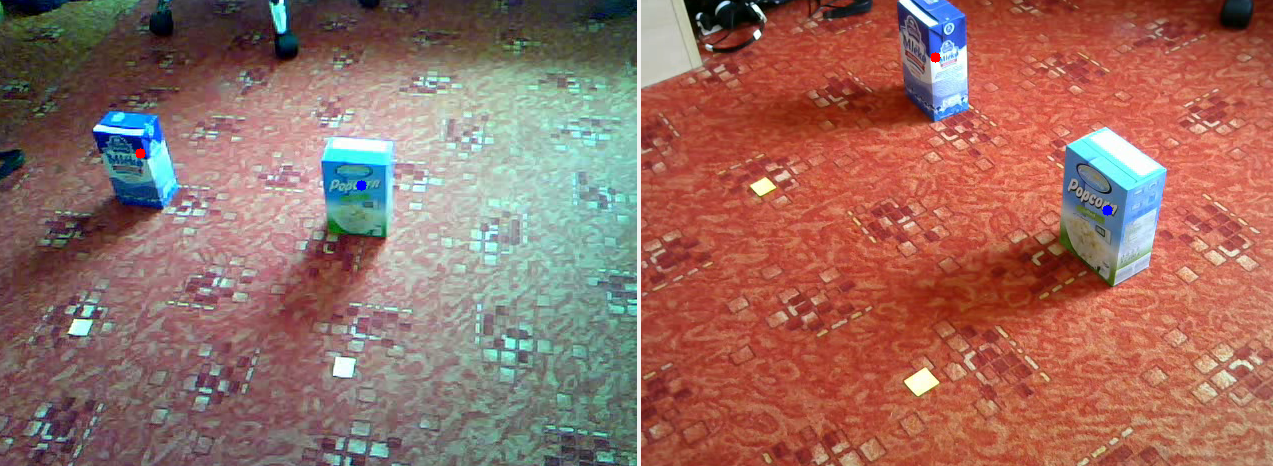
\includegraphics[width=\linewidth]{img/experiments/two-objects.png}
\caption{Initialization of the two objects}
\label{fig:two-init}
\end{figure}

\begin{figure}
\centering
\begin{subfigure}{0.48\linewidth}
	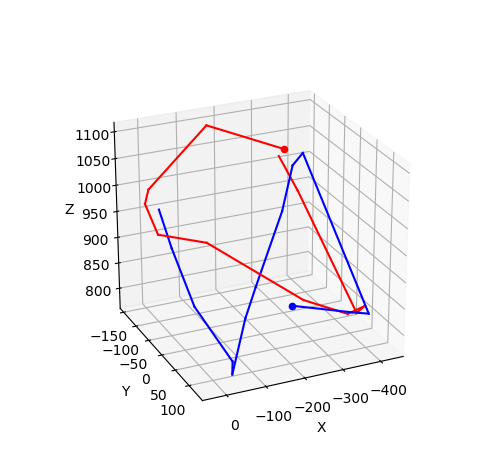
\includegraphics[width=\linewidth]{img/experiments/trajectories1.png}
\end{subfigure}
\begin{subfigure}{0.48\linewidth}
	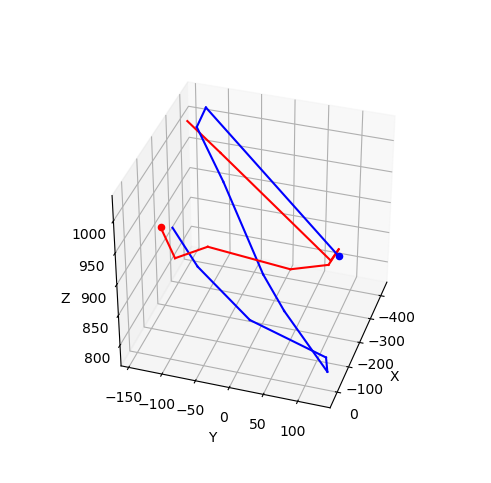
\includegraphics[width=\linewidth]{img/experiments/trajectories2.png}
\end{subfigure}
\caption{Sample trajectories from tracking two objects}
\label{fig:two-trajectories}
\end{figure}

\chapter*{Conclusion}
\addcontentsline{toc}{chapter}{Conclusion}

This thesis proposed a system for object localization in the 3D space.

The primary goal of the thesis was to provide a step by step guide for the task
of the localization of an object in 3D. We achieved the goal by describing
a whole problem and solving it step by step in this thesis.

The thesis started with an overview of the calibration process, explaining the
essential elements of the calibration. We presented a short introduction to
calibration routines used by OpenCV, and we also described the results
obtained by this process.

We implemented detection-based trackers such as \simback{}, \hsv{} and \patt{}.
We explored available trackers in the open-source libraries. These trackers
from the OpenCV and Dlib are sequence-based. We proposed several statistics for
comparison of the trackers. We tested all trackers on several setups, measuring
their speed and accuracy. We also explored their abilities to track multiple
objects and to recover from occlusion. We presented the results in
well-organized tables and provided images for better understanding concepts.

As a next step, we explained how the projection matrices are computed. We
explained their importance in the projection of a point from 3D space to a 2D
view of each camera. The chapter also contains a description of simple
triangulation method. The method shows us how to obtain a position of the
object in 3D space if the projection matrices and the positions in the images
are available.

When all previous steps were covered, we tested the proposed system in several
environments and the settings. We studied the accuracy of the system by static
experiments and computing the estimated distances between the points and
comparing it to real values. In the end, we also provided experiments focusing
on overall experience when using the application.

The application can calibrate automatically using a chessboard pattern, track
one or more objects with a chosen tracker, display the results of the
localization live. Furthermore, it can work with the recordings instead of the
live camera views. The data from the calibration and localization are
automatically saved.

Several areas can be explored in further work. While testing the application,
we noticed a noise in some specific axis. Additional work could explore the
cause of the noise and possible methods to eliminate it. We also explored, that
the precision for the objects further away from the camera is lower compared to
the precision of the closer ones. The question remains, which parameters of our
setup influence this precision and how much. A suitable extension to this
project would be the use of more cameras and explore if this setup improves the
precision.

In the end, we consider the application usable in practice. The results are not
precise enough to provide reliable results in a precision of millimeters but
usable in many cases.


%%% Bibliography
%%% Bibliography (literature used as a source)
%%%
%%% We employ bibTeX to construct the bibliography. It processes
%%% citations in the text (e.g., the \cite{...} macro) and looks up
%%% relevant entries in the bibliography.bib file.
%%%
%%% The \bibliographystyle command selects, which style will be used
%%% for references from the text. The argument in curly brackets is
%%% the name of the corresponding style file (*.bst). Both styles
%%% mentioned in this template are included in LaTeX distributions.

\bibliographystyle{plainnat}    %% Author (year)
% \bibliographystyle{unsrt}     %% [number]

\renewcommand{\bibname}{Bibliography}

%%% Generate the bibliography. Beware that if you cited no works,
%%% the empty list will be omitted completely.

\bibliography{bibliography}

%%% If case you prefer to write the bibliography manually (without bibTeX),
%%% you can use the following. Please follow the ISO 690 standard and
%%% citation conventions of your field of research.

% \begin{thebibliography}{99}
%
% \bibitem{lamport94}
%   {\sc Lamport,} Leslie.
%   \emph{\LaTeX: A Document Preparation System}.
%   2nd edition.
%   Massachusetts: Addison Wesley, 1994.
%   ISBN 0-201-52983-1.
%
% \end{thebibliography}


%%% Figures used in the thesis (consider if this is needed)
\listoffigures

%%% Tables used in the thesis (consider if this is needed)
%%% In mathematical theses, it could be better to move the list of tables to the beginning of the thesis.
%\listoftables

%%% Abbreviations used in the thesis, if any, including their explanation
%%% In mathematical theses, it could be better to move the list of abbreviations to the beginning of the thesis.
% \chapwithtoc{List of Abbreviations}

%%% Attachments to the bachelor thesis, if any. Each attachment must be
%%% referred to at least once from the text of the thesis. Attachments
%%% are numbered.
%%%
%%% The printed version should preferably contain attachments, which can be
%%% read (additional tables and charts, supplementary text, examples of
%%% program output, etc.). The electronic version is more suited for attachments
%%% which will likely be used in an electronic form rather than read (program
%%% source code, data files, interactive charts, etc.). Electronic attachments
%%% should be uploaded to SIS and optionally also included in the thesis on a~CD/DVD.
%%% Allowed file formats are specified in provision of the rector no. 13/2017.
\appendix
%\chapter{Attachments}

%\section{First Attachment}
\chapter{User documentation}
\label{ch:user-documentation}

The purpose of this project is to propose and implement a system for object
localization using a stereo vision -- two cameras. The system computes relative
position of the cameras to each other using a calibration pattern. Then the user
selects the object to track. Different algorithms can be used for tracking.
The tracking algorithms available are detection-based and also sequence-based.
When the object is found in the view of the both cameras, a position in three
dimensional space is estimated. 
This part of the documentation is focused on the end user. We introduce
installation details and manual for program usage.

\section{Installation guide}
This section documents the process of downloading until running the program.

\subsection{Downloading the code}
The code is available at \url{https://github.com/JankaSvK/thesis}.

\subsection{Hardware requirements}
The software was tested on a system with Intel(R) Core(TM) i5-7300HQ CPU
(2.50GHz, 2496 MHz, 4Core), 16GB RAM running Microsoft Windows 10 Enterprise.
Minimal requirements are lower, but the computation power reflects on frequency
of getting localization results. Also, we tested the program on the Ubuntu
16.04.

Two cameras are needed. We tested using a Logitech V-U0018 and Genius
Slim 1322AF. A laptop camera may be used too. Requirements for the cameras
are at least $640\times320$ px resolution and 20 FPS. We advise to turn off the
autofocus, as it changes the focal length.

\subsection{Dependencies}
The following packages are required to run the application. We also provide
versions of packages used to create and test our implementation.

\begin{center}
\begin{tabular}{l l}
	package	&	version 	\\ \hline
	Python	&	3.4.0 		\\
	NumPy	&	1.13.3 		\\
	OpenCV-contrib	&	3.4.0 	\\ 
	Matplotlib &	2.1.1 		\\
	Tkinter	&	8.6 		\\
	PIL (with ImageTk module)	&	1.1.7 		\\
	dlib	&	19.10.0
\end{tabular}
\end{center}

You can easily check the installed versions by running \verb+checkVersions.py+ in
the directory \verb+helpers/+, which is located in the root of the repository.

\section{First run}

In the folder \verb+program/+ we find an entry point for our application
\verb+Main.py+. The text in this chapter is written with assumption that
current directory is the directory \verb+program/+. After starting the
application a window will show up (displayed in Figure \ref{fig:application}).
With no options provided, the program will run on the first two cameras
available.

\begin{figure}
	\frame{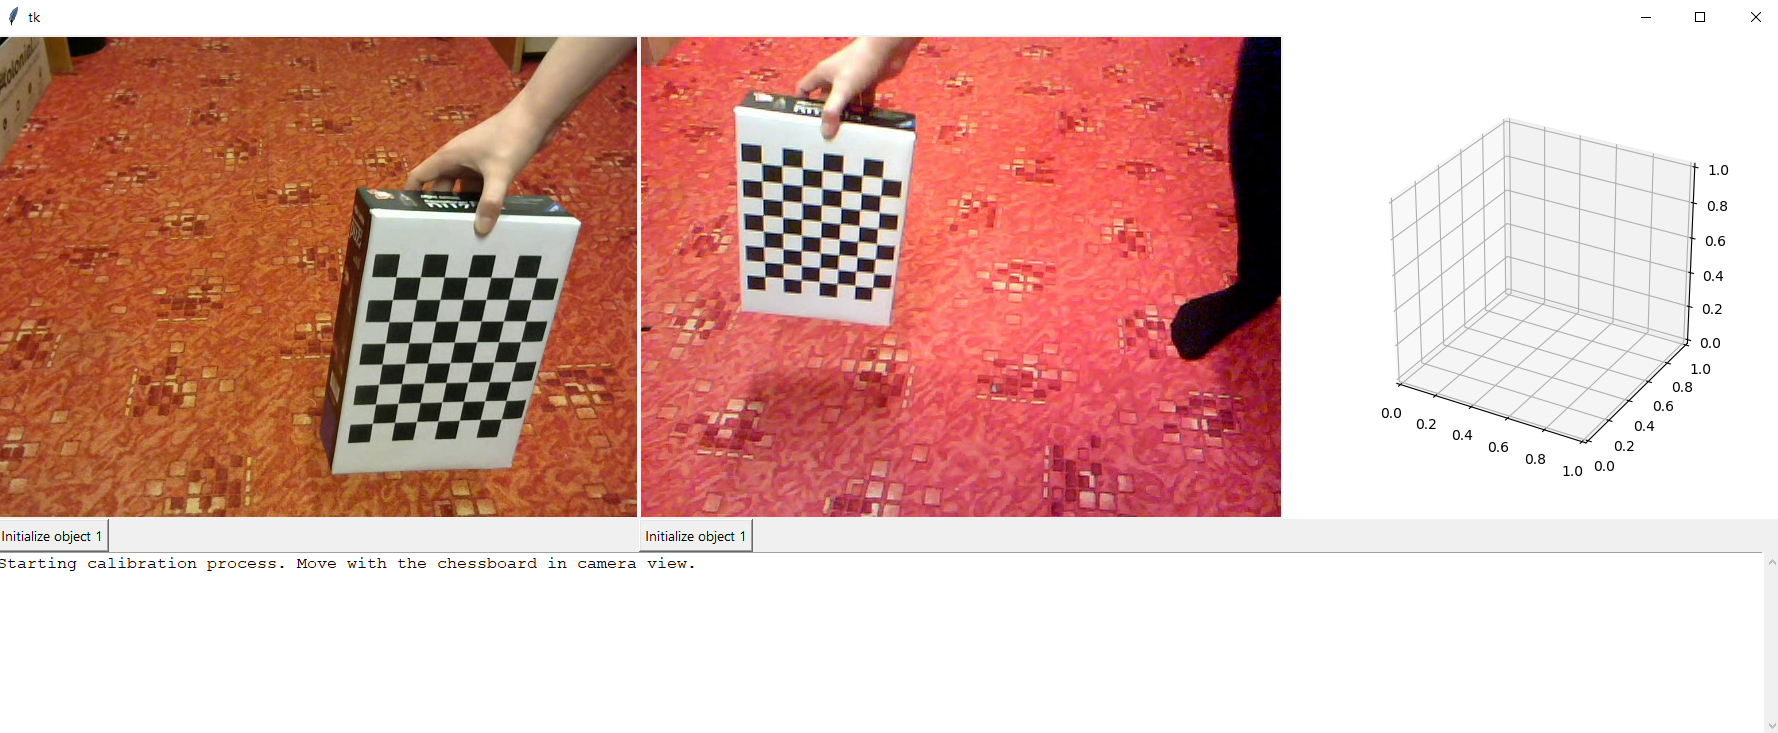
\includegraphics[width=\linewidth]{img/application.png}}
	\caption{Application window}
	\label{fig:application}
\end{figure}

\subsection{Calibration}
As a first step, calibration is expected. We need a calibration pattern --
chessboard (example in the Figure \ref{fig:chessboard}), which could be
printed. For given chessboard, edit values in \verb+program/Config.py+. Change
the value of \verb+chessboard_inner_corners+ to a number of \emph{inner}
corners of your chessboard. For example, classic chessboard 8 $\times$ 8
squares has only 7 $\times$ 7 inner corners, so we enter a tuple \verb+(7, 7)+
as a number of inner corners. Also change \verb+chessboard_square_size+ to the
size of your square in millimeters. It is important to check, if printed
chessboard has squares, not rectangles, since the printer can slightly scale
the image while preprocessing for printing.  Moreover, calibration assumes it
is a planar object, so glue it to the box or another solid object.

For calibration we have to provide a rich set of views of the chessboard. It is important
to move with it and to capture it from various angles, distances and in different
parts of the image. A richer set of views increases robustness of the calibration.

After each successful calibration step you will be notified in the console.
After successful stereo calibration, estimated distance between the cameras
will be printed. If it does not correspond to the reality, consider
a recalibration. If it still did not helped, the user can increase the number of
images needed for calibration in the configuration file (be careful, the computation
time may increase).

If the calibration finished successfully, the calibration results will be
automatically saved in \verb+program/calib_results/+. The files will be saved
into three directories, regarding if it is stereo or mono calibration. In case
of mono calibration, it will be stored in the folder of corresponding camera.
The hierarchy is displayed in the Figure \ref{fig:hierarchy-calib}. The naming
convention for these files is
\verb+{year}-{month}-{day}-at-{hour}-{minute}.json+, where the date and time
specify the moment when the calibration finished.

\begin{figure}
\dirtree{%
.1 calib{\_}results/.
.2 stereo{\_}calib{\_}results/.
.2 1/.
.2 2/.
 }
 \caption{Hierarchy of the directory with saved calibration results}
 \label{fig:hierarchy-calib}
\end{figure}

\subsection{Selecting the objects}
After successful calibration (calibrated with chessboard, or loaded from a
file), the user can initialize the trackers. Under each view of the camera, a button
for each object is located.

For tracker initialization, click on the button. The next two clicks in the
view of the camera, will specify the bounding box for the object. After
initializing trackers in both cameras, localization will automatically start.

If the tracker lost the object, the message is displayed in the camera
view. Note that, not all trackers are able to recognise losing the object.

\subsection{Localization}

After initialization of the trackers, localization will start automatically.
The results are displayed in the graph on the right. We can rotate the graph by
grabbing it by mouse in its window. The dot represents the current position and
the line represent the trajectory.

Results from localization are automatically saved at the end of the program in
\verb+program/localization_data/+. The naming convention for the files includes
the date and time, when was the program closed, i.e it has following form:
\verb+{year}-{month}-{day}-at-{hour}-{minute}-{object_id}.json+.

Saved localization data consists of the four columns separated by tabs. Each
line represents successful localization. In the first column is the time. In the
rest three columns coordinates are stored (x, y, z).

\section{Extras}

Different options may be passed to the program (\ref{code:options}). In case no option
is passed, the program runs on first two available cameras. Firstly, calibration for
each camera is done and then stereo calibration. As a tracker \verb+KCF+ is used by default.

\begin{figure}
\lstset{basicstyle=\ttfamily\footnotesize,breaklines=true,frame=lrtb}
\lstinputlisting[label={code:options}, caption={Available options}]{options.txt}
\end{figure}

\subsection{Notes for options}
\begin{itemize}
\item\emph{Videos} -- only AVI formats are accepted.
\item\emph{Trackers} -- as \verb+TRACKER+ may be used a name of implemented tracker.
Allowed tracker names are: 
\verb+BOOSTING+,
\verb+CORRELATION+,
\verb+HSV+,
\verb+KCF+,
\verb+MEDIANFLOW+,
\verb+MIL+,
\verb+MOSSE+
\verb+PATTERNMATCHING+,
\verb+SIMPLEBACKGROUND+,
\verb+TLD+.
\item\emph{Calibration results} -- calibration results from previous runs may be
used by specifying path to the file.
\item\emph{Chessboard} -- the expected format is for example
\verb+--chesboard=7,8,22+, where the first two number specify number of inner
corners and third is the length of the square side in millimeters.
\end{itemize}

\subsection{Capturing the videos} 

We provide additional script to capture and save videos. The script will
automatically capture video from all available cameras and save it into
\verb+captured_videos+. The capturing can be exited by pressing the key "q".
The script is available in \texttt{helpers/video\_capture.py} from the root
directory of the repository.  

\subsection{Sample scenarios}

\texttt{python3 Main.py} -- runs the application on first two available cameras
\newline
\texttt{python3 Main.py --video1=path/file.avi --video2=path/file.avi} -- runs the application on the videos instead of the cameras
\newline
\texttt{python3 Main.py --tracker=CORRELATION} -- use a correlation tracker
\newline
\texttt{python3 Main.py --chessboard=7,8,22} -- using a chessboard pattern with $7\times8$ inner corners, each has 22 millimeters long side
\newline
\texttt{python3 Main.py -o2} -- setting to track two objects

\chapter{Implementation internals}

%In this chapter we provide an overview of the whole application. The motivation
%is to give you an idea how the program is working and help you to get oriented
%in the code.
%
%\section{Application parts}
%This application has few different parts. All of them have own file and
%sometimes even own thread for processing.
%
%\subsubsection*{Start}
%
%\subsubsection*{ApplicationProcess}
%
%\subsubsection*{Cameras provider}
%
%\subsubsection*{Graphical user interface}
%
%\subsubsection*{Calibrations provider}
%
%\subsubsection*{Trackers provider}
%
%\subsubsection*{Localization provider}
%
%\section{Adding a new tracker}
%

\chapter{How to run experiments}

In thesis, we mentioned many different experiments. In this chapter we provide
a description how to run them by yourself. All dependencies are required.

\section{Tracker's experiments}

All tracker's experiments are located in the directory
\verb+program/experiments/trackers+. The experiments can be started by \verb+trackers{\_}experiments.py+. First argument of the script chooses the scenario for the experiment.

\subsection*{Speed and accuracy}

\verb+trackers{\_}experiments.py 1+

This experiments runs all trackers at the each frame of the video. To compute
an inaccuracy, we use SIMPLEBACKGROUND tracker as the representative tracker
(displayed with the red bounding box).

At the end, results for all trackers are displayed. The first columns specifies
the tracker, the second represents FPS (more described in the chapter Tracker)
and the third the inaccuracy.

\verb+trackers{\_}experiments.py 2+

The second scenario consists of the same experiment, with the orange cap on the
top of the robot, to provide results also for HSV tracker.

\subsection*{Under occlusion}

\verb+trackers{\_}experiments.py 3 tracker_id+

To test a behavior of the trackers under occlusion, we provide an experiment 3.
The reslts from this experiment were obtained by human eye. If the object is
lost, the message is outputed to standard output.

Admissible \verb+tracker{\_}id+ is from \verb+0+ to \verb+8+.

\subsection*{Tracking multiple objects}

\verb+trackers{\_}experiments.py 4 tracker_id+

The fourth experiment focuses on tracking multiple objects. Again, the results were
evaluated by the human. 

Admissible \verb+tracker{\_}id+ is from \verb+0+ to \verb+8+.

\verb+trackers{\_}experiments.py 5 tracker_id+

The same experiment as previous, now with changed objects to be onecolor for
the HSV tracker.


\section{Localization experiment}

\chapter{Additional results}

\begin{table}[h!]
\centering
\begin{tabular}{|r|r|r|r|r|}
\hline
From    & To    & Real length (mm) & Computed length(mm) & Error (\%) \\
\hline
\hline
\input{distances-2.txt}
\hline
\end{tabular}
\label{table:distances-second}
\caption{Results of the experiment focused on the distances}
\end{table}

\openright
\end{document}
